%%% Basic document setup %%%
\documentclass[12pt, letterpaper]{report}
\title{Template}
\author{Anrich Tait}
\date{\today}


%%% Packages %%%
\usepackage{graphicx}	%%% Include images
\graphicspath{{images/}}%%% Where your images are stored (relative to main file)
\usepackage{xeCJK}		%%% Include japanese/chinese/korean
\usepackage{amsmath} 	%%% Math related
\usepackage{xcolor}
\usepackage{float}
\usepackage{geometry}
\usepackage{fancyhdr}
\usepackage{hyperref}
\setCJKmainfont{Source Han Sans JP}
\setCJKsansfont{Source Han Sans JP}
\definecolor{titlepagecolor}{cmyk}{1,.60,0,.40}
\definecolor{namecolor}{cmyk}{1,.50,0,.10}
\hypersetup{colorlinks=true,linkcolor=black,filecolor=magenta,urlcolor=cyan}

\begin{document}

\begin{titlepage}
\newgeometry{left=7.5cm} %defines the geometry for the titlepage
\pagecolor{titlepagecolor}
\noindent
\color{white}
\makebox[0pt][l]{\rule{1.3\textwidth}{1pt}}
\par
\noindent
\textbf{\textsf{コース:}} \textcolor{namecolor}{\textsf{Japanese Self-study}}
\vfill
\noindent
{\huge \textsf{Japanese Notebook}}
\vskip\baselineskip
\noindent
\textsf{作家: Anrich Tait}
\end{titlepage}
\restoregeometry % restores the geometry
\nopagecolor% Use this to restore the color pages to white

\tableofcontents
\begin{abstract}
My self-study Japanese notes.
\end{abstract}

\chapter{Basics}

\section{Basics of timing:}
\begin{enumerate}
	\item Japanese is a moratimed language. Every character occupies the same
		length of time. There is no word stress.
	\item There are 5 vowel characters: \\
		あ = a\\
		い = i\\
		う = u\\
		え = e\\
		お = o\\

\end{enumerate}

\section{Unique sounds of Japanese}
\begin{enumerate}
	\item R is pronounced more like a mix between "r" and "l".
\end{enumerate}

\clearpage
\section{Word order:}
	English word order is Subject, verb, object (SVO), where as in Japanese
		it is subject, object, verb (SOV).\\\\
			Consider the following sentences:\\
			English: I ate an apple (remove article "an" for simplicity)\\
			Japanese: 私りんご食べました. or Watashi ringo tabemashita. 
atashi ringo tabemashita

\begin{center}
\begin{tabular}{|c|c|c|} 
 \hline
 Watashi & ringo & tabemashita. \\ 
 私 & りんご & 食べました. \\ 
 I & apple & ate.\\ 
 \hline
\end{tabular}
		\end{center}
		Notice how the English word order changed with the object now coming 
		second in the sentence.

\section{Topic vs Subject Prominence}
\begin{enumerate}
	\item English is a subject prominent language, meaning that the subject is 
		generally more important than the rest of the sentence. The key piece
		of information about that sentence.
	\item Japanese is a topic prominent language. So what is being done is more
		important than who did the action. Therefore if the subject has already
		been established in a conversation/text then it is common to ommit the
		subject completley.
\end{enumerate}

\subsection{Ommision of the Subject}
Consider the previous example of:\\\\
English: I ate an apple.\\
Japanese: 私がりんごを食べました. Watashi ga ringo o tabemashita.

\chapter{Writing System:}
There are three kinds of characters in Japanese:
\begin{enumerate}
	\item Hiragana: Represents sounds and has a more round shape than other character sets.
		Hiragana is used for conjugation endings, function words and native Japanese words
		not covered in kanji.
	\item Katakana: Also represents sounds but has more straight lines than hiragana and is
		used mainly for writing loanwords and foreign names. For example the Japanese word
		for "television" is writtin in katakana as "テレビ". 
	\item Kanji: Also known as Chinese characters, these represent not only sounds but also
		meanings. Kanji is mostly used for nouns and the stems of verbs and adjectives.
\end{enumerate}

\section{Hiragana:}
\subsection{Basic Syllables:}

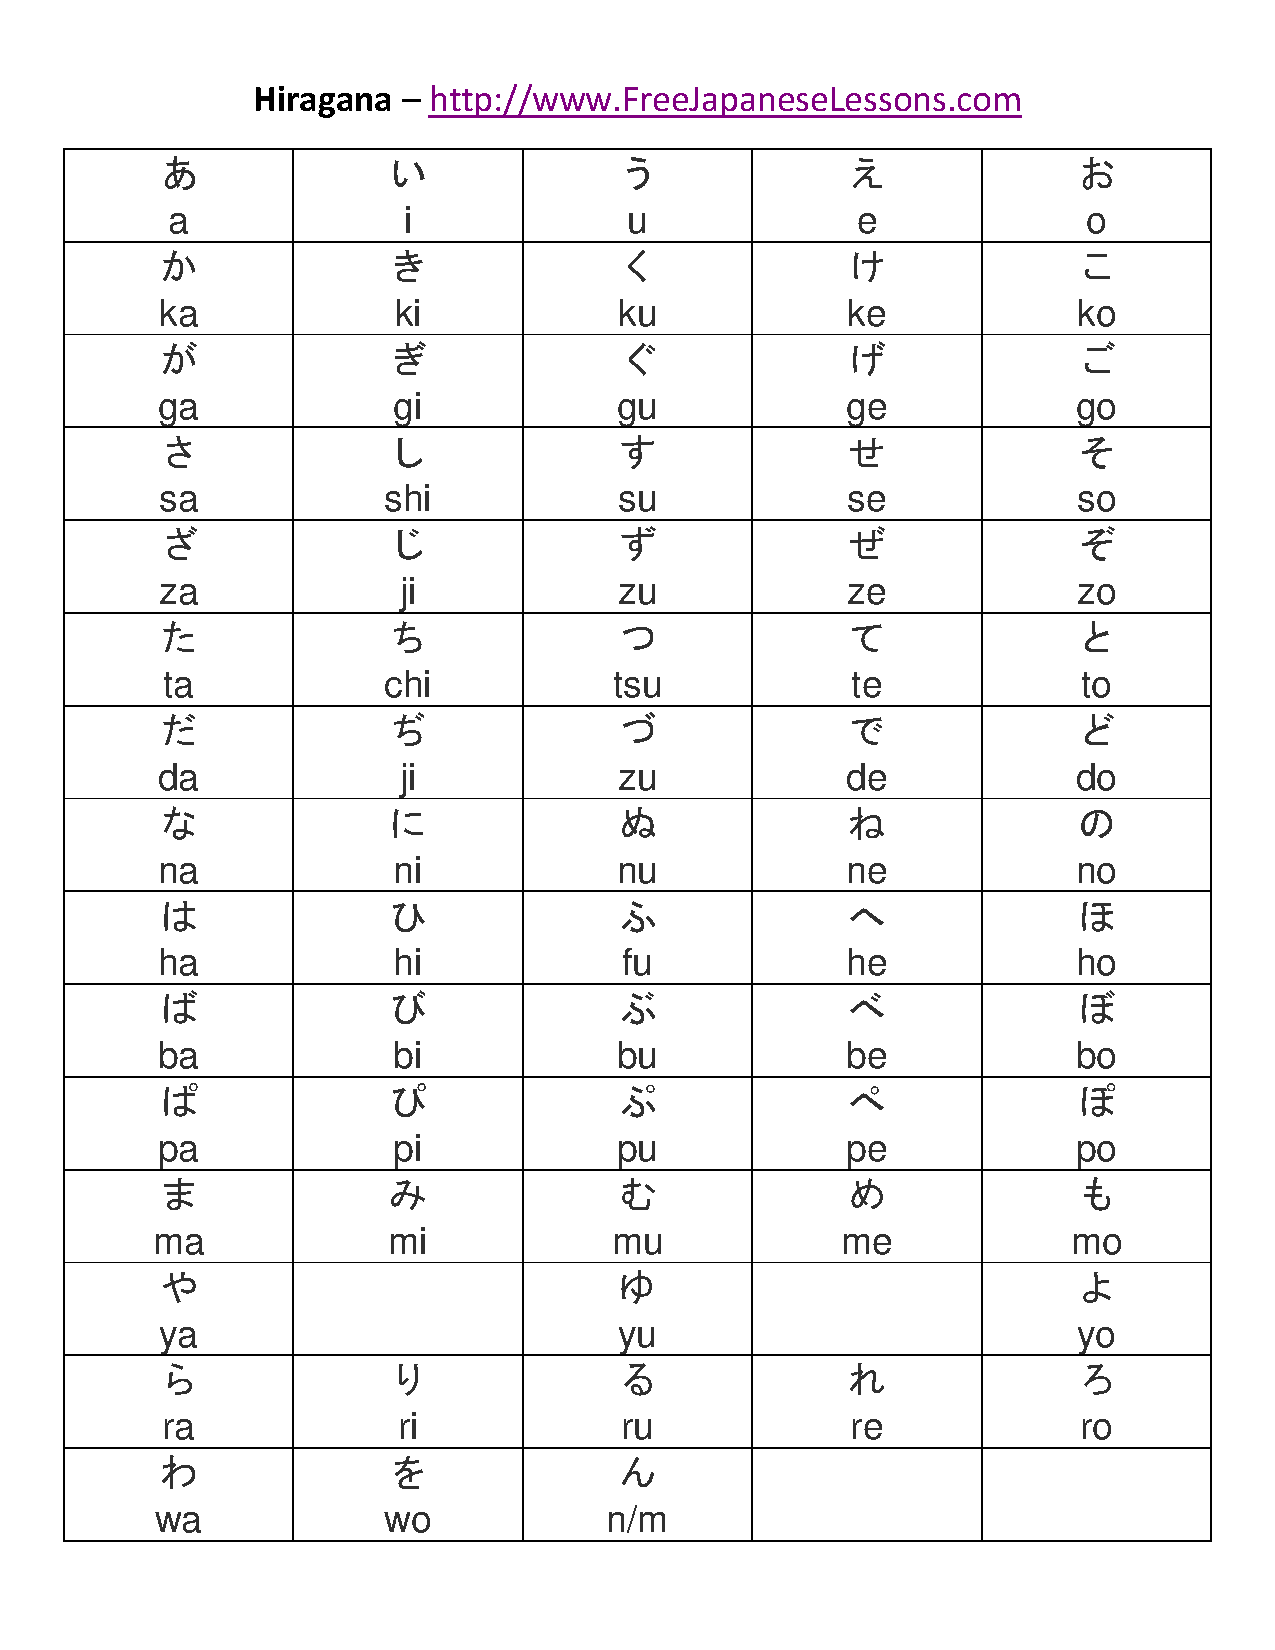
\includegraphics[width=0.75\textwidth]{printable-hiragana-chart}










\chapter{Vocab list:}
\begin{enumerate}
	\item ありがとう = Thank you\\
		arigato
	\item すみません = Excuse me/I'm sorry\\
		sumimasen
	\item トイレ = Bathroom\\
		toire
	\item 駅 = Train station\\
		eki
	\item ホテル = Hotel\\
		hoteru
	\item コンビニ = Convenience store
		konbini
	\item おばあさん = Grandmother\\
		o ba a sa n
	\item (name of place) はどこですか = Where is (name of place)?\\
		wa doko desu ka\\
		"wa" (は) marks the place as subject of sentence\\
		"doko" (どこ) means "where"\\
		"desu" (です) roughly translates to "is" (also "be")\\
		"ka" (か) creates a question\\
	\item わさび = wasabi\\
		wasabi
	\item 
\end{enumerate}













\end{document}
